\documentclass{article}

\title{Building 3D Dense Reconstructions using LiDAR from a Walking Robot}
\author{Marcelo Gennari do Nascimento \\ Wadham College, University of Oxford}
\date{\today}

\usepackage{setspace}
\usepackage{graphicx}
\usepackage[labelfont=bf]{caption}
\usepackage{amsmath}
\graphicspath{ {images/}}
\doublespacing

\begin{document}
	\pagenumbering{gobble}

	\maketitle

	\newpage
	\section*{Acknowledgments}
	\thispagestyle{empty}

	I like to aknowledge ...

	\clearpage
	\newpage

	\begin{abstract}
		Abstract text goes here
	\end{abstract}

	\newpage
	\tableofcontents

	\newpage
	\pagenumbering{arabic}
	\section{Introduction}
	\paragraph{}
	Autonomous robots are going to be one of the major achievements of science to the benefit of the public. Autonomy though depends on two main problems that are tightly related to each other: Localization and Mapping. The first concerns the problem of mapping the environment given a prior robot's trajectory. Most of the time though, neither the trajectory nor the map is known a priori.
	
	\paragraph{}
	Since the 1986 IEEE Robotics and Automation Conference, researchers have framed the general problem of Simultaneous Localization and Mapping (SLAM) as the ``holy grail" of modern robotics \cite{SLAMPartI}. A reliable solution to this problem would make autonomy one step closer to reality. Since the conference, a number of algorithms have been developed that successfully tackle SLAM, each of them with their advantages and drawbacks.

	\paragraph{}
	This project is concerned with putting together state of the art algorithms for SLAM and reconstruction systems to reliably and effiiciently build a 3D map of an environment with LiDAR data from a walking robot without any prior map or prior trajectory available. The success of this project would contribute to making the usage of mobile robots for tasks such as search and rescue and exploration one step closer to reality.

	\subsection{Aim of the Project}
	\subsection{ Organisation of the Report}

	\newpage
	\section{Literature Review}
	\subsection{Simultaneous Localization and Mapping (SLAM)}
	\paragraph{}
	SLAM is the problem of whether it is possible for a mobile robot to create a globally consistent map of an environment and localize itself on it without prior knowledge of the map \cite{SLAMPartI}\cite{Cadena}. Building a map of an environment is a crucial step towards autonomy, since planning and control assume prior knowledge of mapping and localization. Mathematically, we can frame SLAM as a Markov Chain, a Bayes Net or a Factor Graph. Defining:
	
	\begin{itemize}
		\item $\mathbf{x_k}$: the pose of the robot (being $\mathbf{X_{0:k}}$ as the poses from time $\mathbf{0}$ to $\mathbf{k}$)
		\item $\mathbf{u_k}$: the odometry measurement ($\mathbf{U_{0:k}}$ as the historical measurements)
		\item $\mathbf{l_k}$: the landmark observation ($\mathbf{L_{0:k}}$ as the historical landmarks)
		\item $\mathbf{c_k}$: the loop closures
	\end{itemize}

	It is possible to formulate the problem of SLAM more formally using both a factor graph or a probabilistic framework:

	\begin{figure}[h]
		\centering
		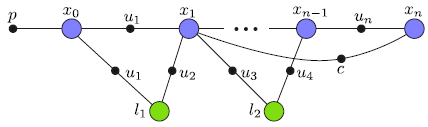
\includegraphics[width=\textwidth,height=\textheight,keepaspectratio]{SLAMFactorGraph.png}
		\caption{SLAM as a Factor Graph. The value $\mathbf{p}$ denotes a prior; $\mathbf{x_n}$ denotes the state vector; $\mathbf{u_n}$ denotes odometry measurements; $\mathbf{c}$ denotes close loops; $\mathbf{l_n}$ denotes landmark positions.}
		\label{fig:slam1}
	\end{figure}
	
	\paragraph{}
	The graph shown in Figure \ref{fig:slam1} is a Factor Graph representation of the dependencies between variables and measurements. A probabilistic framework can then be extracted from it. 
	\begin{equation}
	P(X,L,U,Z,C) \alpha\prod_{i=1}^{M}P(x_i|x_{i-1}, u_i)\prod_{k=1}^{K}P(z_k|x_{i_k},l_{j_k})\prod_{w=1}^{W}P(x_i|x_{i_w}, c_w)
	\label{probSLAMeq}
	\end{equation}
	For the rest of this chapter, it will be assumed that the data association problem is solved and the indices $i_w$ and $i_k$ are known. 

	\paragraph{}
	Theoretically, the mathematical formulation of the SLAM has been shown that it is indeed feasible to build a nondivergent map with no prior information, so it is widely accepted that in theoretical grounds, SLAM is a solved problem \cite{SLAMPartI}\cite{Cadena}\cite{CsorbaThesis}\cite{938381}. However, there are computational and algorithmic challenges that hinders the development of a real-time implementation system that performs SLAM. This problem gets even more complicated when considering unstructured environments and large scale maps \cite{SLAMPartII}.
	
	\paragraph{}
	Modern analysis of the SLAM algorithms have shown that \cite{doi:10.1177/1729881416669482}

	\paragraph{}
	There are three main implementations of SLAM: Kalman Filtering and Extended Kalman Filtering (with early works such as proposed by R. Smith \cite{Smith:1990:EUS:93002.93291}), Rao-Blackwellized Particle Filtering (most notably with FastSLAM \cite{Montemerlo02fastslam:a}) and Information Matrix (with the now state-of-the-art work of iSAM from Michael Kaess \cite{Kaess08tro}).

	\subsubsection{Kalman Filtering}
	\paragraph{}
	As one of the first implementations to appear to solve the problem of SLAM, (Extended) Kalman Filtering approach makes two assumptions when formulating the probabilistic SLAM: the process model and the observation model.
	\begin{minipage}{.45\linewidth}
		\centering
		\begin{equation*}
		\begin{split}
		\mathbf{Process\ Model:} \\ 
		x_i = f(x_i) + w_i
		\end{split}
		\end{equation*}
	\end{minipage}
	\begin{minipage}{.5\linewidth}
		\centering
		\begin{equation*}
		\begin{split}
		\mathbf{Observation\ Model:} \\ 
		z_i = h(x_{i_k}, l_{j_k})+ + v_k
		\end{split}
		\end{equation*}
	\end{minipage}

	\paragraph{}
	As a consequence, the probability distributions can be 


	\paragraph{}
	It is know that the Kalman Filter approach requires storage of the order of $O(N^2)$ (where $N$ is the number of features), and for a classic implementation of the algorithm, it also requires computational power of the order of $O(N^2)$ \cite{CsorbaThesis}. New methods for computing the covariances (which cause the squared dependence) by exploring state augmentation, partitioned updates and sparsity in the matrices have demonstrated faster solutions, thus requiring less computational power \cite{SLAMPartII}.

	\subsubsection{Particle Filtering}
	\subsubsection{Information Matrix}
	\subsection{Iterative Closest Points (ICP)}
	\subsection{3D Reconstruction Systems}

	\newpage
	\section{System Pipeline}
	\paragraph{}
	The pipeline for the overall system can be seen below. It consists of 4 modules: (I) First odometry estimates (based on either Visual Odometry or Wheel Odometry); (II) Laser Odometry (using Simona Nobili's AICP); (III) Loop closure detection and Graph Optimization (using iSAM); (IV) 3D dense volumetric reconstruction (using BOR\textsuperscript{2}G-CUBES).

	\paragraph{}
	These 4 modules are broken down in two parts: the first part is concerned about solving the SLAM problem, which outputs a reliable trajectory and map. The second part is concerned about inputting that to a 3D reconstruction system (which in this case if BOR\textsuperscript{2}G-CUBES) to build the environment volumetrically.

	\newpage
	\section{SLAM Solution}
	\subsection{First Odometry Measurements}
	\subsection{Laser Odometry}
	\subsection{Loop Closure Detection}
	\subsection{Graph Optimization}

	\newpage
	\section{Integration with BOR\textsuperscript{2}G-CUBES}
	
	\newpage
	\section{Conclusion}

	\newpage
	\bibliography{4YPReportBibl}
	\bibliographystyle{ieeetr}

\end{document}